\section{预备知识}

\subsection{再生核希尔伯特空间Reproducing Kernel Hilbert Space}
RKHS由函数构成, 在希尔伯特空间中使用"核技巧"将一组数据映射到一个高维空间, 这个高维空间就是可再生核希尔伯特空间. 

在低维空间中不能线性分割的点集, 通过转化为高维空间中的点集时, 很有可能变为线性可分的.

\paragraph{核方法}
在低维空间中不能线性分割的点集, 通过转化为高维空间中的点集时, 从而变为线性可分的.
\paragraph{核技巧}
在原始空间找到一个函数$K(x_i,x_j)$使得$K(x_i,x_j) = <\phi(x_j),\phi(x_j)>$.
如果这个函数存在, 那么我们只需要在低维空间里计算函数$K(x_i,x_j)$的值即可, 而不需要先把数据映射到高维空间, 再通过复杂的计算求解映射后的内积. 这种简化计算的方法被称为核技巧(The Kernel Trick)

\subsubsection{常用的核函数}

主要有以下几种:

\paragraph{线性核} 其实就是没有映射 $\kappa \left ( x_{1},x_{2} \right ) = \left \langle x{1},x{2} \right \rangle$

\paragraph{高斯核函数}使用最为广泛, 把原始特征映射到无穷维.
 $\kappa \left ( x_{1},x_{2} \right ) = \exp \left ( -\frac{\left | x_{1}-x_{2} \right |^{2}}{2\sigma ^{2}} \right )$

 \paragraph{多项式核函数}, 把数据映射到$C_{n+d}^{n}$维.
$\kappa \left ( x_{1},x_{2} \right ) = \left ( \left \langle x_{1},x_{2} \right \rangle  +R\right )^{d}$

\paragraph{再生核希尔伯特空间}
在一定条件下, 可以找到对应于这个希尔伯特空间上唯一的再生核函数 $K$, 其满足以下几点:\\
对任意固定$x_0$属于$X$, 有$K(x,x_0)$作为$X$的函数属于$H$;\\
对任意$x$属于$X$,$f(.)$ 属于$H$, 有$f(x) = {<f(.),K(.,x)>_{H}}$, 则称$K(.,x)$为$H$的再生核,$H$是以$K(.,x)$为再生核的希尔伯特空间, 简称再生核希尔伯特空间. 

\paragraph{希尔伯特空间定义流程}

向量空间$\rightarrow$内积空间$\rightarrow$赋范向量空间$\rightarrow$度量空间$\rightarrow$Banach空间$\rightarrow$Hilbert空间

\begin{description}
    \item[向量空间Vector Space]:满足加法和标量乘操作的集合
    \item[范数向量空间Normed Vector Space]:定义了向量长度的向量空间$\left || x \right || = <x,x>$
    \item[度量空间Metric Space]:定义了两个点的距离的集合
    \item[巴拿赫空间Banach Space]:一个完备的范数向量空间
    \item[内积空间Inner Product Space]:指在定义域上可进行内积运算法操作的向量空间
    \item[希尔伯特空间Hilbert Space]:当一个内积空间满足通过内积空间可推导出范数空间, 且是完备的, 那么这个内积空间就是希尔伯特空间. 

\end{description}
\paragraph{RKHS的两个定理}
\begin{itemize}
    \item 
    一个希尔伯特空间H是一个再生核希尔伯特空间, 当且仅当它有一个再生核
    \item 
    对于给定的再生核希尔伯特空间, 其再生核是唯一的. 
\end{itemize}


\paragraph{经典RKHSs技术的三个问题} \cite{peifer2020sparse}
 \begin{itemize}
     \item 首先, 它们需要先验知识, 而这在许多应用中是不现实的.此外, RKHS的选择会影响溶液的形状和平滑度, 从而影响其性能.
     \item其次, RKHS不具备处理异构平滑度的能力, 也就是说, 函数在其领域的某些部分是平滑的, 但在其他部分变化迅速.
     \item最后, 随着训练样本中数据点的增加, 评估这些方法解的计算复杂度增加, 使得这些技术在许多应用中不可行.
    
 \end{itemize}
 虽然核学习、局部核自适应和稀疏性已被用于解决这些问题, 但这些方法中的许多都是计算密集型的或放弃了最优性保证.
 可以利用RKHSs中的一个新的积分表示来解决这些问题, 这些RKHSs允许任意中心和每个中心的不同内核.为了解决复杂性问题, 我们然后将函数估计问题写成一个稀疏函数程序, 它显式地最小化导致低复杂性解决方案的表示法的支持.尽管这些问题具有非凸性和无限维数, 但我们证明利用对偶性可以准确有效地解决这些问题, 并在模拟和实际数据中说明了这种新方法.
%% 这儿总结一些比较重要的数学概念、定理等.
\subsection{梯度下降}
\subsubsection{随机梯度下降Stochastic gradient descent}
随机梯度下降(通常缩写SGD)是一种迭代方法用于优化的目标函数与合适的光滑性质(例如可分化或subdifferentiable).它可以被看作是随机逼近的梯度下降优化, 因为它取代了实际梯度(从整个计算数据集通过其估计值(从数据中随机选择的子集计算)).特别是在大数据应用中, 这减轻了计算负担, 实现更快的交易迭代, 但收敛速度略低. 
\begin{algorithm}  
    \caption{ Stochastic  General decent method}  
    \begin{algorithmic}
\STATE{ Choose an initial vector of parameters  w and learning rate  $\eta$ .Repeat until an approximate minimum is obtained:
\begin{itemize}
    \item Randomly shuffle examples in the training set.
    \item For $  i=1, 2, ..., n$,  do:
    $w:=w-\eta \nabla Q_{i}(w)$ 
\end{itemize}
}
    \end{algorithmic}  
   \end{algorithm}  
\subsubsection{ADMM 交替向量乘子法}
ADMM也是增广拉格朗日函数, 只是由一个变量变成两个变量
$$L(x, z;\lambda)= f(x) + g(z) + \lambda ^T(Ax + Bz - c) + \rho/2 * ||Ax + Bz -c ||^2$$
固定其中两个变量, 去更新第三个变量的值

$ \text{step1}: x^{k+1} = arg \min_x L(x, z^k, \lambda^k) \\
\text{step2}: z^{k+1} = arg min_z L(x^{k+1}, z, lambda^k) \\
\text{step3}: \lambda ^ {k+1} = \lambda^k + \rho (Ax + Bz - c) \\$
于是问题就变化为了如何求解 $arg min_x L$
\subsubsection*{decentralized SGD去中心化 SGD}
 

Decentralized Federated Learning via SGD over Wireless D2D Networks (H Xing,  O Simeone,  S Bi)

\subsection{张量分解}
张量(tensor)是一个多维的数据存储形式, 数据的的维度被称为张量的阶.它可以看成是向量和矩阵在多维空间中的推广, 向量可以看成是一维张量, 矩阵可以看成是两维的张量.
\subsubsection{CP分解}
将高维的张量分解成为Rank-One Tensors的和.
$X \approx [ \!  [ \mathbf{A, B, C} ]\!] \equiv \sum_{r=1}^{R}a_r \circ b_r \circ c_r$

这里$\circ$指的是外积.
\subsubsection{Tucker 分解  }

Tucker分解将张量分解为一组矩阵和一个小的核心张量.

 $X = G \times_1 A^{(1)} \times_2  A^{(2)} \dots \times_N A^{(N)}= [\! [  G:A^{(1)},  A^{(2)},  A^{(N)}   ] \! ] $

\subsection{Dataset shift 数据集偏移}
数据集偏移是指训练和测试分布不同时的情况.
数据集偏移主要发生在有监督的机器学习范式和半监督学习的混合范式内.
数据集移位的问题可能源于利用输入特征的方式, 选择训练和测试集的方式, 数据稀疏性, 由于非平稳环境而导致的数据分布移位, 以及源于各层内激活模式的变化.深度神经网络.
数据集移位的表现形式:协变量移位、先验概率转移、概念转变、内部协变量移位(协变量移位的重要子类型)

\subsubsection{有状态和无状态}
有状态就是有数据存储功能.有状态对象(Stateful Bean), 就是有实例变量的对象 , 可以保存数据, 是非线程安全的.在不同方法调用间不保留任何状态.

无状态就是一次操作, 不能保存数据.无状态对象(Stateless Bean), 就是没有实例变量的对象.不能保存数据, 是不变类, 是线程安全的.
 
\subsection{激活函数}
激活函数在神经元中非常重要的.为了增强网络的表示能力和学习能力, 激活函数需要具备以下几点性质:
\begin{enumerate}
\item 连续并可导(允许少数点上不可导)的非线性函数.可导的激活函数可以直接利用数值优化的方法来学习网络参数.
\item 激活函数及其导函数要尽可能的简单, 有利于提高网络计算效率.
\item 激活函数的导函数的值域要在一个合适的区间内, 不能太大也不能太小, 否则会影响训练的效率和稳定性.
\end{enumerate}
\subsubsection{Sigmoid型函数}
常用的Sigmoid 型函数有Logistic 函数和Tanh 函数.
\paragraph{Logistic函数}
$$\sigma(x)=\frac{1}{1+\exp(-x)}$$
和感知器使用的阶跃激活函数相比, Logistic 函数是连续可导的, 
装备了Logistic激活函数的神经元具有以下性质:
\begin{enumerate}
    \renewcommand{\labelenumi}{(\theenumi)}
 \item 其输出直接可以看作概率分布, 使得神经网络可以更好地和统计学习模型进行结合. 
 \item 其可以看作一个软性门(Soft Gate), 用来控制其他神经元输出信息的数量.
\end{enumerate}

\textbf{优点}:
\begin{enumerate}
    \renewcommand{\labelenumi}{(\theenumi)}
\item 便于求导的平滑函数;
\item 能压缩数据, 保证数据幅度不会有问题;
\item 适合用于前向传播.
\end{enumerate}

\textbf{缺点}:
\begin{enumerate}
    \renewcommand{\labelenumi}{(\theenumi)}
    \item 容易出现梯度消失的现象 
   \item Sigmoid的输出不是0均值 的:这会导致后层的神经元的输入是非0均值的信号, 这会对梯度产生影响.以 $f=\mathrm{sigmoid}(wx+b)$为例,  假设输入均为正数(或负数), 那么对w的导数总是正数(或负数), 这样在反向传播过程中要么都往正方向更新, 要么都往负方向更新, 导致有一种捆绑效果, 使得收敛缓慢.
    \item 幂运算相对耗时 
\end{enumerate}
\paragraph{求导}
$ \frac{\rho \sigma(x)}{\rho(x)}=\sigma(x)(1-\sigma(x))$
​	 
\paragraph{Tanh函数}
$$\tanh(x)=\frac{\exp(x)-\exp(-x)}{\exp(x)+\exp(-x)} $$
Tanh 函数可以看作放大并平移的Logistic 函数, 其值域是(-1,  1).
$$\tanh(x) = 2 \sigma (2x)-1$$

\begin{figure}[!ht]
    \centering
    % \label{ }
    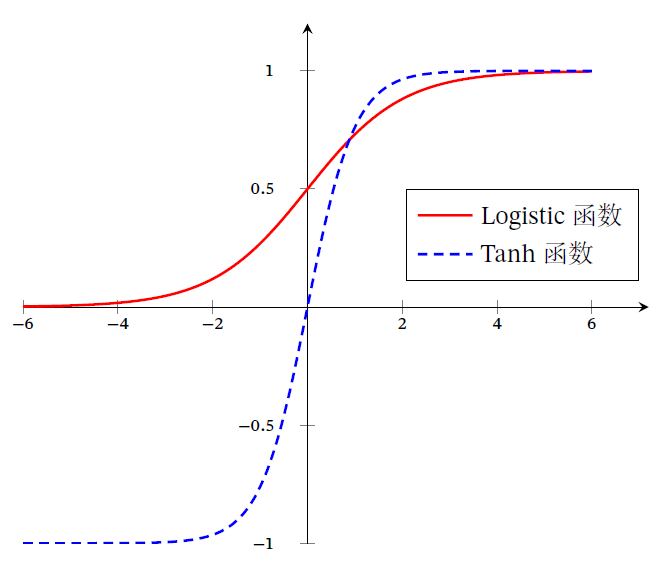
\includegraphics[width=0.4\textwidth]{sigmoid_function.png}
    \caption{Logistic 函数和Tanh 函数}
\end{figure}

\textbf{优缺点}:
Tanh函数是0均值的, 解决了Sigmoid函数的非zero-centered问题, 但是它也存在梯度消失和幂运算的问题.


\subsubsection{整流线性单位函数(Rectified Linear Unit,  ReLU)}
ReLU 实际上是一个斜坡(ramp)函数, 定义为
$$\mathrm{ReLU}(x)=
\left\{ 
\begin{array}{c}    x \\    0  \\   \end{array}
\right. =\max(0, x)
$$
\begin{figure}[!ht]
    \centering
    \includegraphics[width=\textwidth]{ReLU}
    \caption{ReLU激活函数}
\end{figure}
\paragraph{求导}
$$\frac{\rho\sigma(x)}{\rho(x)}=1-\sigma^2(x)$$

\textbf{优点}:
\begin{enumerate}
    \renewcommand{\labelenumi}{(\theenumi)}
    \item   ReLu的收敛速度比 sigmoid 和 tanh 快(梯度不会饱和, 解决了梯度消失问题);
     \item  计算复杂度低, 不需要进行指数运算;
     \item 适合用于后向传播.
\end{enumerate}

\textbf{缺点}:
\begin{enumerate} 
    \renewcommand{\labelenumi}{(\theenumi)}
\item  ReLU的输出不是zero-centered; 
\item  Dead ReLU Problem(神经元坏死现象):某些神经元可能永远不会被激活, 导致相应参数永远不会被更新(在负数部分, 梯度为0).

\textbf{产生原因}:
\begin{itemize}
    \item 参数初始化问题
    \item 学习率太高导致在训练过程中参数更新太大
\end{itemize}
 \textbf{解决方法}:采用Xavier初始化方法, 以及避免将学习率设置太大或使用adagrad等自动调节学习率的算法.
\item ReLU不会对数据做幅度压缩, 所以数据的幅度会随着模型层数的增加不断扩张.
\end{enumerate}
\paragraph{Leakly  ReLU函数}
用来解决ReLU带来的神经元坏死的问题, 可以将0.01设置成一个变量a, 其中a由后向传播学出来.但是其表现并不一定比ReLU好.

\begin{align*}
\mathrm{ELU}(x)=&
\left\{ 
\begin{array}{c c}    
    x  \ & \text{if} \  x>0 \\    
    \gamma_i x \ & \text{if} \ x \leqslant 0  \\   
\end{array} 
\right. \\
=& \max(0, x)+\gamma_i \min(0, x)
\end{align*}
其中$\gamma_i$为$x \leqslant 0 $时函数的斜率

\paragraph{ELU函数(指数线性函数)}
ELU有ReLU的所有优点, 并且解决了 Dead ReLU问题, 输出的均值接近0(zero-centered).但是计算量大, 其表现并不一定比ReLU好.
\begin{align*}
    \mathrm{ELU}(x)= &
    \left\{ 
    \begin{array}{c c}    
        x  \ & \text{if} \  x>0 \\    
        \gamma(\exp(x)-1) \ & \text{if} \ x \leqslant 0  \\   
    \end{array} 
    \right. \\
    = & \max(0, x)+\gamma_i \min(0, \gamma(\exp(x))-1)
    \end{align*}
      

\subsubsection{Entropy熵}
在信息论中, 熵用来衡量一个随机事件的不确定性.
 自信息(Self Information)表示一个随 机事件所包含的信息量. 一个随机事件发生的概率越高, 其自信息越低.如果-一个事件必然发生, 其自信息为0.
 对于一一个随机变量X (取值集合为X , 概率分布为$p(x,  x \in \mathcal{X})$, 当X=x
 时的自信息$I(x)$定义为
 \begin{equation}
      I(x)=- \log p(x).
 \end{equation} 
 
 在自信息的定义中, 对数的底可以使用2、自然常数$e$或是10.当底为2时, 自信息的单位为bit;当底为e时, 自信息的单位为nat.
 对于分布为$p(x)$的随机变量X , 其自信息的数学期望, 即熵$H(X)$定义为
 
 \begin{equation}
    \begin{split}
 H(X) &= \mathbb{E}_x\left[  I(x)\right] \\
 &= \mathbb{E}_x \left[  -\log p(x) \right] \\
 &=\sum_{x \in \mathcal{X}}p(x) \log p(x)    
\end{split}
 \end{equation}
 其中$ 0 \log 0= 0 $.
 熵越高, 则随机变量的信息越多;熵越低, 则随机变量的信息越少

\subsubsection{Cross Entropy交叉熵}
对于分布为$p(x)$的随机变量, 熵$H(p)$表示其最优编码长度.交叉熵(Cross Entropy)是按照概率分布$q$的最优编码对真实分布为$p$的信息进行编码的长度, 定义为 
\begin{equation}
 \begin{split}
        H(p, q)&= \mathbb{E}_p \left[ -\log q(x) \right]  \\
        &= - \sum_x p(x) \log q(x) 
 \end{split}
\end{equation}
 
在给定$p$的情况下, 如果$q$ 和$p$ 越接近, 交叉熵越小;如果$q$ 和$p$ 越远, 交叉熵就越大.


\subsection{神经网络}
“神经网络是由具有适应性的简单单元组成的广泛并行互连的网络, 它的组织能够模拟生物神经系统对真实世界物体所作出的交互反应”[Kohonen,  1988].

神经网络中最基本的单元是神经元模型(neuron), 最简单的神经元模型是“M-P神经元模型”.
树突对应于输入部分, 每个神经元收到n个其他神经元传递过来的输入信号, 这些信号通过带权重的连接传递给细胞体.
细胞体分为两部分, 前一部分计算总输入值(即输入信号的加权和), 后一部分先计算总输入值与该神经元阈值的差值, 然后通过激活函数的处理, 产生输出从轴突传送给其它神经元.
\begin{figure}
    \centering
    \label{MP_Model}
    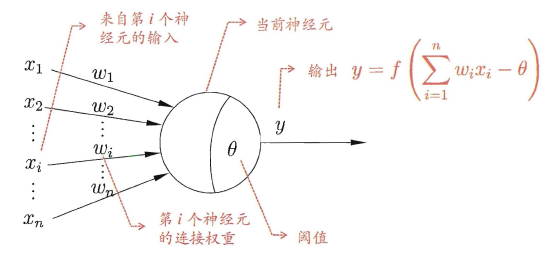
\includegraphics[width=0.9\textwidth]{MP_Modle.png}
    \caption{M-P神经元模型}
\end{figure}

神经元模型最理想的激活函数也是阶跃函数, 但阶跃函数不连续, 常采用Sigmoid函数来近似.

\subsubsection{感知器}
感知机(Perceptron)是由两层神经元组成的一个简单模型, 但只有输出层是M-P神经元, 即只有输出层神经元进行激活函数处理, 也称为功能神经元;输入层只是接受外界信号(样本属性)并传递给输出层(输入层的神经元个数等于样本的属性数目), 而没有激活函数感知机的输出层应该可以有多个神经元, 从而可以实现多分类问题, 同时两个模型所用的参数估计方法十分不同.

\begin{figure}
    \centering
    \label{MP}
    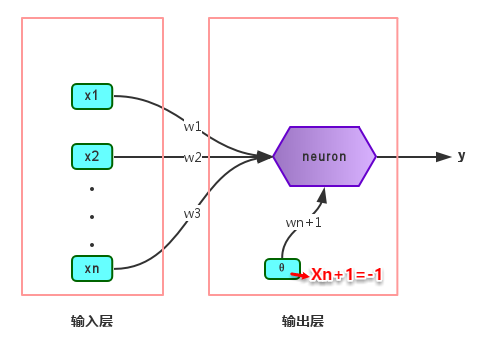
\includegraphics[width=0.5\textwidth]{simple_perceptron.png}
    \caption{简单感知机}
\end{figure}
\newpage
\paragraph{感知机学习算法} 给定个样本的训练集${(x^{(n)}, y^{(n)}}^N_{n1}$, 其中$y(n)\in {+1, -1}$, 感知器学习算法试图找到一组参数$\mathbf{w}^{\star}$, 使得对于每个样本$(x^{(n)}, y^{(n)}$有
\begin{equation}
    y^{(n)} \mathbf{w}^{\star \mathrm{T} }  \mathcal{x}^{(n)}> 0,  \forall n \in \{ 1, ..., N \}
\end{equation}
\begin{figure}
    \centering
    \label{algorithm_perceptron}
    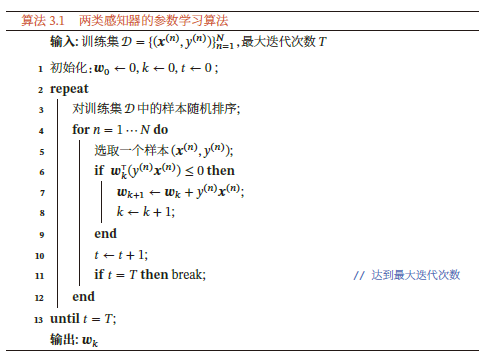
\includegraphics[width=0.9\textwidth]{algorithm_perceptron.png}
    \caption{两类感知机学习算法 }
\end{figure}

\paragraph{感知器的收敛性} 
 感知器收敛性:给定训练集 $D = {x(), y(0)}$令R是训练集
中最大的特征向量的模, 即$$R = \max_n \|x^{(n)}\|$$
如果训练集D线性可分, 两类感知器的参数学习算法3.1的权重更新次数不
超过$\frac{R^2}{\gamma^2}$次.

\paragraph{几种常见的线性模型对比} 
\begin{figure}
    \centering
    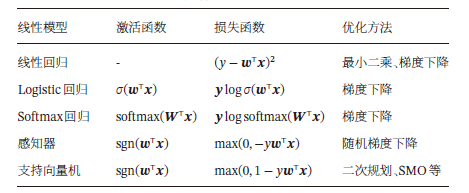
\includegraphics[width=0.7\textwidth]{linear_model.png}
    
\end{figure}
\newpage
\paragraph{不同损失函数的比较}
\begin{figure}
    \centering
    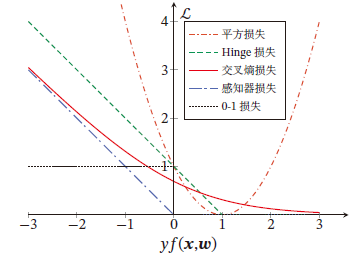
\includegraphics[width=0.7\textwidth]{loss_function.png}
    \caption{不同损失函数的比较}
\end{figure} 
一个好的损失函数应该随着$yf(\mathbf{x;w})$的增大而减少.

\subsubsection{分类问题总结}
分类问题中的决策函数需要输出离散值或是标签的后验概率.线性分类模型一般是一
个广义线性函数, 即一个或多个线性判别函数加上一个非线性激活函数.在Logistic 回归和Softmax 回归中, y 为类别的one-hot 向量表示;在感知器和支持向量机中, y 为$\{+1, -1\}$.



\subsubsection{数据集}
如果已经有了一个比较大的标注数据集, 想要完成一个有监督模型的测试, 那么通常使用均匀随机抽样的方式, 将数据集划分为训练集、验证集、测试集, 这三个集合不能有交集, 常见的比例是8:1:1. 三个集合都是同分布的. 
训练集就是用来训练参数的. 而验证集基本是在每次epoch完成后, 测试当前模型的准确率. 
对于一个模型来说, 其参数可以分为普通参数和超参数. 除强化学习外, 普通参数是可以被训练所更新. 超参数不在梯度下降的更新范围内, 需要人工根据验证集调节.所以在广义上, 验证集参与了人工调参的过程, 需要一个没有经过的训练的集合, 就是测试集来测试最终准确率. \citep{training_validation_test_Su}


\subsection{前馈神经网络}
在前馈神经网络中, 不同的神经元属于不同的层, 每一层的神经元可以接受到前一层的神经元信号, 并产生信号输出到下一层.第0层叫做输入层, 最后一层叫做输出层, 中间的叫做隐藏层, 整个网络中无反馈, 信号从输入层到输出层单向传播, 可用一个有用无环图表示.

前馈神经网络也成为多层感知器(Mutlti-Layer Perceptron, MLP).但是这种叫法并不准确, 因为前馈神经网络其实是由多层Logistic回归模型(连续的非线性模型)组成, 而不是有多层感知器模型(非连续的非线性模型)组成.

下图为简单的前馈神经网络图:

\begin{figure}[!ht]
    \centering
    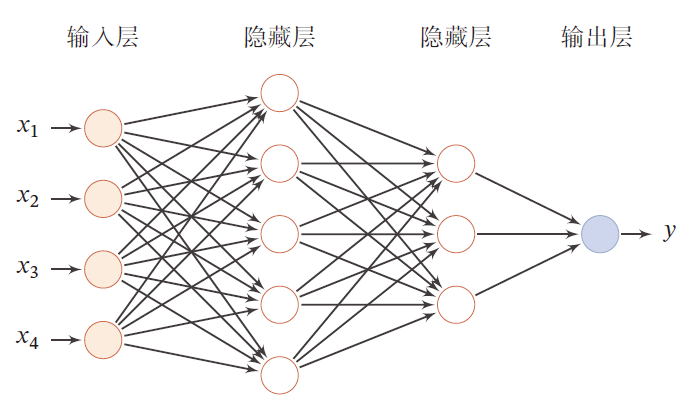
\includegraphics[width=0.6\textwidth]{FNN}
    \caption{前馈神经网络图}
\end{figure} 


神经网络中涉及的多个记号:
\begin{table}[!ht]
    \renewcommand{\arraystretch}{1.35}  
    \centering
    \begin{tabular}{cc}
        \toprule
        记号 & 含义 \\
        \midrule
        $L$ &表示神经网络的层数\\
$m^{(l)}$&表示第$ l$ 层神经元个数\\
$f_l ( \cdot ) $&表示第$ l $层神经元的激活函数\\
$W^{(l)}$   &表示第$ l-1$ 层到第 l 层的权重矩阵\\
$b^{(l)}$   &表示第$ l-1$ 层到第 l 层的偏置\\
$z^{(l)}$   &表示第 $l$ 层神经元的净输入(净活性值)\\
$a^{(l)}$   &表示第$l$层的神经元输出(活性值)\\
        \bottomrule
    \end{tabular}
\label{tabel:NerualNetwork_mark}
\caption{神经网络中涉及的记号}
\end{table}

神经网络的信息传播公式如下 
\begin{gather*}
 z^{(l)} = W^{(l)}   a^{(l-1)} + b^{(l)}\\
 a^{(l)} = f_l(z^{(l)})
\end{gather*} 
 可以合并写为 :
$$z^{(l)}=W^{(l)} f_{(l-1)} (z^{(l-1)})+b^{^{(l)}}  $$
或者 
$$a^{(l)} = f_l(W^{(l)} a^{(l-1)} + b^{(l)})$$
这样神经网络可以通过逐层的信息传递, 得到网络最后的输出$a^{(l)}$.整个网络可以看做一个符合函数$$\phi (x; W, b)$$
将向量x作为第一层的输入$a^0$, 将第 l 层的输入$a^0$,  将第L层的输出$a^{(l)}$ 作为整个函数的输出.
$$ x = a^0 \rightarrow z^1 \rightarrow a^1 \rightarrow z^2 .... \rightarrow a^{L-1} \rightarrow z^{(l)} \rightarrow a^{(l)} = \phi (x;W, b)$$
其中W,  b表示网络中所有层的连接权重和偏置. 
\paragraph{参数学习}
如果采用交叉熵损失函数, 对于样本$(x, y)$, 其损失函数为:
$$L(y, \hat{y}) = -y^T log (\hat{y})$$, 
其中 y 属于${0, 1}^T$为标签y对应的one-hot向量.

给定训练集$D={(x^{(n)}, y^{(n)},  N>=n>=0}$, 将每个样本$x^n$ 输入给前馈神经网络, 得到网络输出为$y^n$, 其在数据集$\mathcal{D}$上的结构化风险函数为:
$$R(W, b)=\frac{1}{N}\sum_{n=1}^{N} L(y^n, \hat{y}^n) + \frac{1}{2}\lambda \left \| W \right \|_F^2$$
 
其中W和b分别表示网络中所有的权重矩阵和偏置向量,  $\|W\|_F^2$ 是正则化项, 用来防止过拟合, $\lambda$是为正数的超参数, $\lambda$越大, W越接近于0.这里的$(\|W\|_F)^2$一般使用Frobenius范数.
 
有了学习准则和训练样本, 网络参数可以通过梯度下降法来进行学习.在梯度下降方法的每次迭代过程中, 第l层的参数$ W^{(l)} $和$ b^{(l)}$ 参数更新方式为:
\begin{gather*}
    W^{(l)} \leftarrow W^{(l)} - \alpha \frac{\partial R(W, b)}{\partial W^{(l)}}=W^{(l)} - \alpha ( \frac{1}{N} \sum_{n=1}^{N}(\frac{\partial L(y^n, \hat{y}^n)}{\partial W^{(l)}}) + \lambda W^{(l)} )\\b^{(l)} \leftarrow b^{(l)} - \alpha \frac{\partial R(W, b)}{\partial b^{(l)}}=b^{(l)} - \alpha ( \frac{1}{N} \sum_{n=1}^{N}(\frac{\partial L(y^n, \hat{y}^n)}{\partial b^{(l)}}) ) 
\end{gather*}
其中$\alpha$为学习率.
梯度下降法需要计算损失函数对参数的偏导数, 如果通过链式法则逐一对每个参数进行求偏导效率比较低.在神经网络的训练中经常使用反向传播算法来高效的计算梯度. 
\subsubsection{反向传播算法}
基于误差的反向传播算法(backpropagation, BP)的前馈神经网络训练过程可以分为以下三步:
\begin{enumerate} 
    \renewcommand{\labelenumi}{(\theenumi)}
\item 前馈计算每一层的净输入$z^{(l)}$ 和激活值 $a^{(l)}$, 直到最后一层
\item 反向传播计算每一层的误差项
\item 计算每一层参数的偏导数, 并更新参数
\end{enumerate}

它利用均方误差和梯度下降的方法来实现对网络连接权值的修改.网络连接权值的修改是为了使误差平方和最小.该算法首先对网络的连接值赋一个小的值, 然后选择一个训练样本来计算相对于这个样本的误差梯度.
\begin{figure}
    \centering
    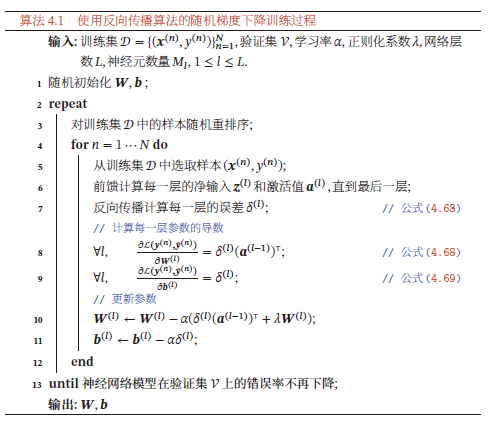
\includegraphics[width=0.7\textwidth]{algorithm_bp.png}
\end{figure} 

\subsubsection{优化问题}
\paragraph{非凸优化问题}
使用非凸的损失函数
如平方误差损失函数和交叉熵损失函数
\paragraph{梯度消失问题}
由于Sigmoid 型函数的饱和性, 饱和区的导数更是接近于0.这样, 误差经
过每一层传递都会不断衰减.当网络层数很深时, 梯度就会不停衰减, 甚至消
失, 使得整个网络很难训练.这就是所谓的梯度消失问题(Vanishing Gradient
Problem), 也称为梯度弥散问题.

\subsubsection{通用近似定理}
通用近似定理( Universal Approximation Theorem) 

令$\Phi(\cdot)$是一个非常数、有界、单调递增的连续函数,  $\mathcal{J}_D$是一个D维的单位超立方体$[0, 1]^D$,  $C(\mathcal{p})$是定义在$\mathcal{J}_D$.上的连续函数集合对于任何-一个函数$f \in C(\mathcal{J}_D)$, 存在一个整数M, 和一组实数$v_m, b_m \in R$以及实数向量$v_m \in R^D, m= 1,  \cdots,  M$ 以至于我们可以定义函数
$$F(x) =2v_m \phi(v_m^T x + b_m)$$
作为函数f的近似实现, 即
$$|F(x)- f(x)|< \upsilon_i \forall x \in (\mathcal{J}_D) $$
其中$ \upsilon > 0$是一个很小的正数.


一个前馈神经网络如果具有线性输出层和至少一层具有任何一种"挤压"性质的激活函数(例如 sigmoid激活函数)的隐藏层, 只要给予网络足够数量的隐藏单元, 它可以以任意的精度来近似任何一个任何定义在实数空间$ R^D$中的有界闭集函数(Borel 函数). 神经网络的通用近似性质也被证明对于其他类型的激活函数, 比如ReLU, 也都是适用的.

学习失败原因:
\begin{itemize}
    \item 用于训练的优化算法可能找不到用于期望函数的参数值.
    \item 训练算法可能由于过拟合而选择了错误的函数.
\end{itemize}
\subsection{循环神经网络}

\textbf{前馈网络的一些不足}
\begin{itemize}
    \item 连接存在层与层之间, 每层的节点之间是无连接的(无循环)
    \item 输入和输出的维数都是固定的, 不能任意改变.无法处理变长的序列数据.
    \item 假设每次输入都是独立的, 也就是说每次网络的输出只依赖于当前的输入.
\end{itemize}

\textbf{循环神经网络}(Recurrent Neural Network, RNN)通过使用带自反馈的神经元, 能够处理任意长度的序列, 比前馈神经网络更加符合生物神经网络的结构.
给定-一个输入序列$x_{1:T} =(x_1, x_2,  .... x_t, .... x_T)$, 循环神经网络通过下面公式更新带反馈边的隐藏层的活性值$h_t$:
$$h_t= f(h_t-1, x_t)$$
其中$h_0= 0, f( \cdot )$为一个非线性函数, 可以是一个前馈网络.
\begin{figure}[!htb]
    \center
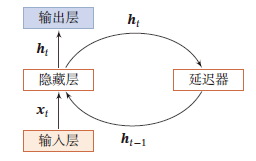
\includegraphics[width=0.7\textwidth]{RNN_sample.png}
\caption{循环神经网络}
\end{figure}


图中“延时器”为一个虚拟单元, 记录神经元的最近一次(或几次)活性值.
\subsubsection{简单循环网络}
Simple Recurrent Network, SRN \citep{elman1990finding} 
 
$$h_t = f(Uh_t-1 +Wx_t + b)$$
\begin{figure}[!htb]
    \center
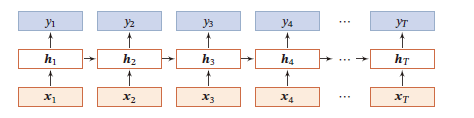
\includegraphics[width=0.7\textwidth]{simple_RNN.png}
\caption{按时间展开的循环神经网络}
\end{figure}


\subsubsection{循环神经网络的计算能力}
循环神经网络的拟合能力十分强大.一个完全连接的循环网络是任何非线性动力系统的近似器.
如果一个完全连接的循环神经网络有足够数量的sigmoid 型隐藏神经元, 它可以以任意的准确率去近似任何一个非线性动力系统

\begin{equation*}
    \begin{split}
        S_t &= g(S_{t-1}, x_t) \\
        y_i & = o(s_t)
    \end{split}
\end{equation*}
其中$S_t$为每个时刻的隐状态, $x_t$是外部输入, $g(\cdot)$是可测的状态转换函数, 
$o(\cdot)$ 是连续输出函数, 并且对状态空间的紧致性没有限制.
 
\begin{figure}[!htb]
    \center
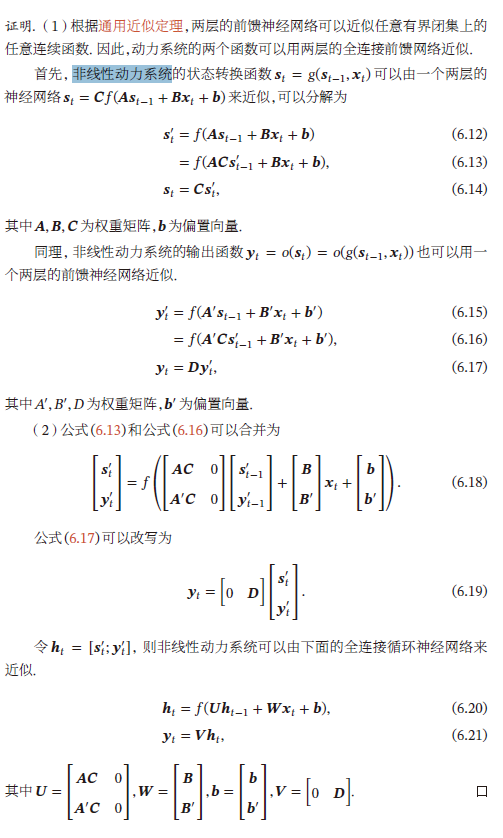
\includegraphics[width=0.8\textwidth]{RNN_univesal.png}
\end{figure}



% \subsubsection{循环神经网络在机器学习中的应用}


 \paragraph{长期依赖(Long-Term Dependencies)问题}
如果相关信息和当前预测位置之间的间隔就相当的大, 在这个间隔不断增大时,  RNN会难以学习到连接如此远的信息. (梯度消失和梯度爆炸)

在序列中, 依赖现象较为明显, 如主谓依赖、名词与动词单复数的依赖. 在较短范围内, 这种依赖能够被传统的语言模型(如n-gram, 神经语言模型)刻画, 但是长距离依赖则是传统语言模型难以刻画的. 长距离依赖是序列建模的重要刻画内容之一.
循环神经网络在进行梯度反向传播时也面临着梯度消失和梯度爆炸问题, 只是表现在时间轴上, 即如果输入序列很长,  梯度难以更新. 



解决: LSTM GRU Attention


\paragraph{序列到类别模式}

输入为序列, 输出为类别.比如在文本分类中, 输入数据为单词的序列, 输出为该文本的类别.

假设一个样本$$ x_{1:T}=(x_1, ...,  x_T)$$ 为一个长度为T的序列, 输出为一个类别 $y \in {1,  2,  \dot C}$.可以将样本x按不同时刻输入到RNN中, 得到不同时刻的隐藏状态 $h_1,  \dots,  h_T$ .可以将 $h_T$看作整个序列的最终表示, 并输入给分类器 $g(\cdot)$进行分类,  $\hat{y}=g(h_T)$

其中 $g(\cdot)$可以是简单的线性分类器如Logistic回归, 或复杂分类器如前馈神经网络.

除了将最后时刻的状态作为小于列表示之外, 还可以对整个序列的所有状态进行平均, 用这个平均状态作为整个序列的表示:
\begin{figure}[!htb]
    \center
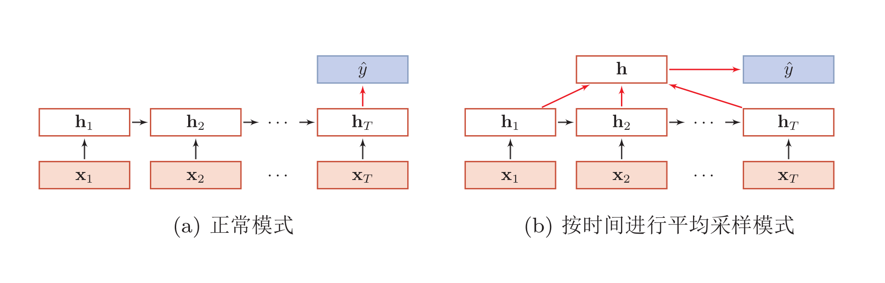
\includegraphics[width=0.8\textwidth]{RNN_model1.png}
\caption{序列到类别模式}
\end{figure}


\paragraph{同步的序列到序列模式}

\begin{figure}[!htb]
    \center
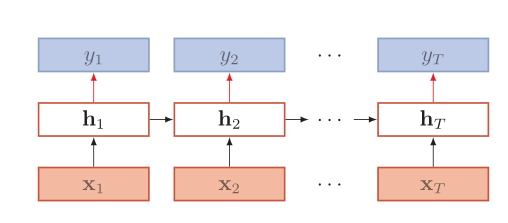
\includegraphics[width=0.8\textwidth]{RNN_model2.png}
\caption{同步的序列到序列模式}
\end{figure}
每一时刻都有输入和输出, 输入序列和输出序列的长度相同, 如词性标注(Part-of-Speech Tagging)中, 每一个单词都需要标注其对应的词性标签.

输入为一个长度为T的序列$$ x_{1:T}=(x_1, ...,  x_T)$$, 输出为序列$y_{1:T}=(y_1, ...,  y_T)$.样本x按不同时刻输入到RNN中, 并得到不同时刻的隐状态$h_1,  \dots,  h_T$ .每个时刻的隐状态$h_t$代表了当前时刻和历史的信息, 并输入给分类器 $g(\cdot)$得到当前时刻的标签 $ \hat{y}_t$ .
$$\hat{y}= g(h_t),  \  \forall t \in [1, T]$$



\paragraph{异步的序列到序列模式}
也称为编码器-解码器(Encoder-Decoder)模型, 输入序列和输出序列不需要严格的对应关系, 也不需要保持相同的长度.类似于机器翻译.

输入为一个长度为T的序列 $ x_{1:T}=(x_1, ...,  x_T)$, 输出长度为M的序列 $ y_{1:T}=(y_1, ...,  y_T)$ .先将样本x按不同时刻输入到RNN中(编码器), 得到其编码 $h_T$ , 然后使用另一个RNN(解码器), 得到输出序列$ \hat{y}_{1:m}$ , 为了建立输出序列之间的依赖关系, 在解码器中通常使用非线性的自回归模型.

\begin{equation}
    \begin{split}
        h_t &= f_1(hp_1, x),   \forall t \in [1, T] \\
    h_{T+t}& = f_2(h_{T+t-1}, \hat{y}_{t-1}),  \forall t\in[1, M]\\
    \hat{y}&= g(h_{T+t}),   \forall t\in[1, M]
    \end{split} 
\end{equation}

其中 $f(\cdot)$ 为编码器和解码器的神经网络,  $g(\cdot)$ 为分类器,  $\hat{Y}_t$为预测输出 $\hat{y}_t$的向量表示.
\begin{figure}[!htb]
    \center
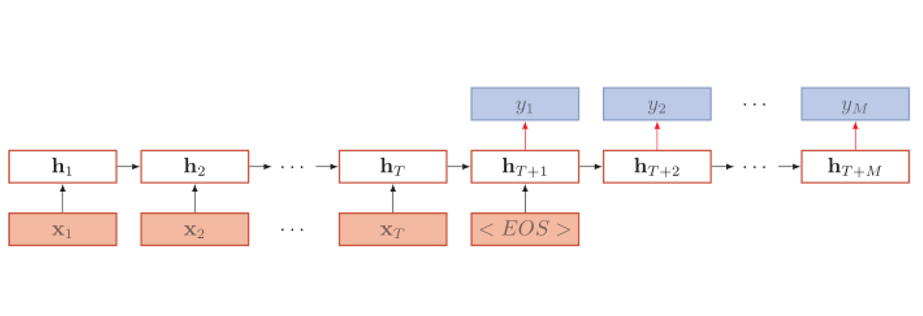
\includegraphics[width=0.8\textwidth]{RNN_model3.png}
\caption{异步的序列到序列模式}
\end{figure}

% \subsubsection{========}

% 将字符打乱顺序普通神经网络无法预测下一个

% \begin{tikzcd}
%     &  \arrow[rd,  "\mathbf{b}^{(l)} \to \mathbf{I}_{m^{(l)}}"] &                                      &                                         & {\partial{L}(\mathbf{y},  \hat{\mathbf{y}})} \arrow[lld,  "\delta^{l}"'] \arrow[d,  "\delta^{l+1}"] &  \\
% \mathbf{a}^{(l-1)} \arrow[rr,  "W_{ij}^{(l)} \to a_{j}^{(l-1)}"'] &                                                          & \sum \mathbf{z}^{(l)} \arrow[r,  "f"] & \mathbf{a}^{(l)} \arrow[r,  "W^{(l+1)}"] & \mathbf{z}^{(l+1)} \arrow[r,  "f"]                                                                &  \\
%     &  \arrow[ru]                                              &                                      &                                         &                                                                             & 
% \end{tikzcd}


% \textbf{RNN应用在知识图谱--图网络}

\subsubsection{简介实现}

\begin{enumerate}
    \item  使用困惑度评价模型. 
    \item  在迭代模型参数前裁剪梯度. 
    \item  对时序数据采用不同采样方法将导致隐藏状态初始化的不同
\end{enumerate}

\subsection{通过时间反向传播}
BPTT 算法将循环神经网络看作一个展开的多层前馈网络, 其中“每一层”对应循环网络中的“每个时刻”, 所有层的参数是共享的, 因此参数的真实梯度是所有“展开层”的参数梯度之和.
% \begin{figure}[!htb]
%     \center
% 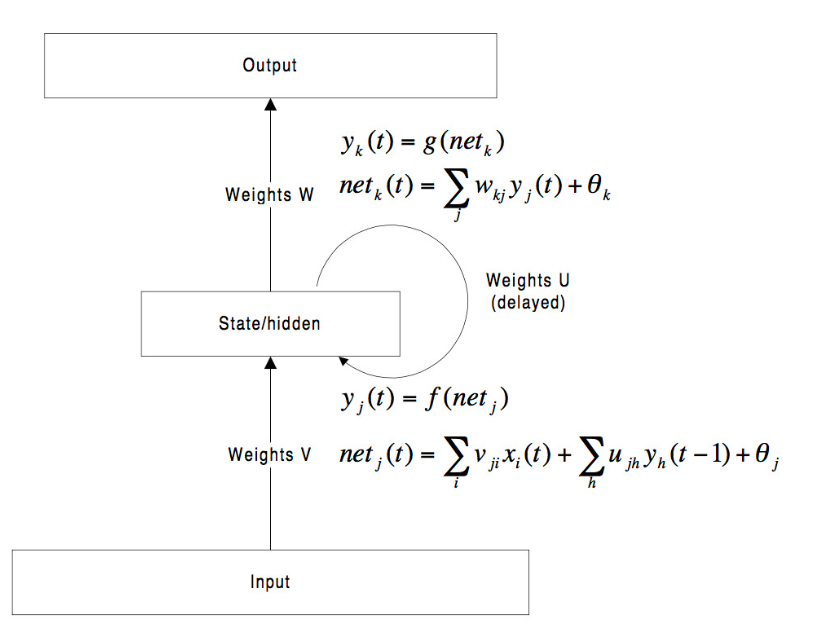
\includegraphics[width=0.6\textwidth]{BPTT.png}
% \caption{BPTT算法}
% \end{figure}
假设
\begin{itemize}
\item 激活函数$\Phi(x)=x$, 
\item t时刻输入$\mathbf{x}_t \in \mathbb{R}^d$, 
\item 标签 $y_t$
\item 隐藏状态 $\mathbf{h}_t \in \mathbb{R}^h$
\item 隐藏层权重 
$$\mathbf{W}_{hx} \in \mathbb{R}^{h \times d}$$
$$\mathbf{W}_{hh} \in \mathbb{R}^{h \times h}$$
\item 输出层权重
$\mathbf{W}_{qh} \in \mathbb{R}^{q \times h}$
\item
t时刻输出$\mathbf{o}_t \in \mathbb{R}^q$, 

$$\mathbf{o}_t = \mathbf{W}_{qh} \mathbf{h}_{t}.$$
\item 
t 时刻损失 $\ell(\mathbf{o}_t,  y_t)$
时间步数为T的损失函数$$L = \frac{1}{T} \sum_{t=1}^T \ell (\mathbf{o}_t,  y_t).$$
\end{itemize}
  
prod运算符将根据两个输⼊矩阵的形状, 在必要的操作(如转置和互换输⼊位置)后对两个输⼊做乘法. 


计算
目标函数有关各时间步输出层变量的梯度 $\partial L/\partial \mathbf{o}_t \in \mathbb{R}^q$
$$\frac{\partial L}{\partial \mathbf{o}_t} =  \frac{\partial \ell (\mathbf{o}_t,  y_t)}{T \cdot \partial \mathbf{o}_t}.$$

有关模型参数$\mathbf{W}_{qh}$的梯度
$$
\frac{\partial L}{\partial \mathbf{W}_{qh}} 
= \sum_{t=1}^T \text{prod}\left(\frac{\partial L}{\partial \mathbf{o}_t},  \frac{\partial \mathbf{o}_t}{\partial \mathbf{W}_{qh}}\right) 
= \sum_{t=1}^T \frac{\partial L}{\partial \mathbf{o}_t} \mathbf{h}_t^\top.
$$
 
有关最终时间步隐藏状态的梯度$\partial L/\partial \mathbf{h}_T \in \mathbb{R}^h$
$$
\frac{\partial L}{\partial \mathbf{h}_T} = \text{prod}\left(\frac{\partial L}{\partial \mathbf{o}_T},  \frac{\partial \mathbf{o}_T}{\partial \mathbf{h}_T} \right) = \mathbf{W}_{qh}^\top \frac{\partial L}{\partial \mathbf{o}_T}.
$$


对于时间步$t < T$, 

目标函数有关时间步$t < T$的隐藏状态的梯度$\partial L/\partial \mathbf{h}_t \in \mathbb{R}^h$需要按照时间步从大到小依次计算:

$$
\frac{\partial L}{\partial \mathbf{h}_t}
= \text{prod}\left(\frac{\partial L}{\partial \mathbf{h}_{t+1}},  \frac{\partial \mathbf{h}_{t+1}}{\partial \mathbf{h}_t} \right)
+ \text{prod}\left(\frac{\partial L}{\partial \mathbf{o}_t},  \frac{\partial \mathbf{o}_t}{\partial \mathbf{h}_t} \right)
= \mathbf{W}_{hh}^\top \frac{\partial L}{\partial \mathbf{h}_{t+1}} + \mathbf{W}_{qh}^\top \frac{\partial L}{\partial \mathbf{o}_t}.
$$

将上面的递归公式展开, 对任意时间步$1 \leq t \leq T$, 我们可以得到目标函数有关隐藏状态梯度的通项公式
$$
\frac{\partial L}{\partial \mathbf{h}_t} 
= \sum_{i=t}^T {\left(\mathbf{W}_{hh}^\top\right)}^{T-i} \mathbf{W}_{qh}^\top \frac{\partial L}{\partial \mathbf{o}_{T+t-i}}.
$$
 
隐藏层中模型参数的梯度$\partial L / \partial \mathbf{W}_{hx} \in \mathbb{R}^{h \times d}$和$\partial L / \partial \mathbf{W}_{hh} \in \mathbb{R}^{h \times h}$. 
$$
\begin{aligned}
\frac{\partial L}{\partial \mathbf{W}_{hx}} 
&= \sum_{t=1}^T \text{prod}\left(\frac{\partial L}{\partial \mathbf{h}_t},  \frac{\partial \mathbf{h}_t}{\partial \mathbf{W}_{hx}}\right) 
= \sum_{t=1}^T \frac{\partial L}{\partial \mathbf{h}_t} \mathbf{x}_t^\top, \\
\frac{\partial L}{\partial \mathbf{W}_{hh}} 
&= \sum_{t=1}^T \text{prod}\left(\frac{\partial L}{\partial \mathbf{h}_t},  \frac{\partial \mathbf{h}_t}{\partial \mathbf{W}_{hh}}\right) 
= \sum_{t=1}^T \frac{\partial L}{\partial \mathbf{h}_t} \mathbf{h}_{t-1}^\top.
\end{aligned}
$$



%  \textbf{偏置项}
\subsection{语言模型}

标准定义:对于语言序列 $w_1, w_2, \dots,  w_n$, 语言模型就是计算该序列的概率, 即 $P(w_1, w_2,  \dots,  w_n)$ .
从机器学习的角度来看:语言模型是对语句的概率分布的建模.
通俗解释:判断一个语言序列是否是正常语句, 即人是否可理解, 例如 $P(I am Light) > P(Light I am)$ .
\paragraph{n元语法}

当序列长度增加时, 计算和存储多个词共同出现的概率的复杂度会呈指数级增加. n 元语法通过马尔可夫假设(虽然并不一定成立)简化了语言模型的计算.这里的马尔可夫假设是指一个词的出现只与前面 n 个词相关, 即 n 阶马尔可夫链(Markov chain of order n).如果 n=1 , 那么有 $P(w_3∣w_1, w_2)=P(w_3∣w_2)$ .如果基于 n-1 阶马尔可夫链, 我们可以将语言模型改写为
$$P(w_1, w_2, \cdots , w_T) \approx \Pi_{t=1}^T P(w_t|w_t-(n-1), \cdots, w_{t-1})$$.
以上也叫 n 元语法(n-grams). 它是基于 n-1 阶马尔可夫链的概率语言模型.当 n 分别为1、2和3时, 我们将其分别称作一元语法(unigram)、二元语法(bigram)和三元语法(trigram).

\subsection{深度循环神经网络}
含有多个隐藏层的循环神经网络, 也称作深度循环神经网络. 下图演示了一个, \textbf{每个隐藏状态不断传递至当前层的下一时间步和当前时间步的下一层}. 

 \begin{figure}[!htb]
    \center
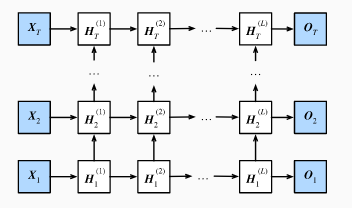
\includegraphics[width=0.6\textwidth]{deep_rnn.png}
\caption{有$L$个隐藏层的深度循环神经网络}
\end{figure}
 

具体来说, 在时间步$t$里, 设小批量输入$\mathbf{X}_t \in \mathbb{R}^{n \times d}$(样本数为$n$, 输入个数为$d$), 第$l$隐藏层($l=1, \ldots, L$)的隐藏状态为$\mathbf{H}_t^{(l)}  \in \mathbb{R}^{n \times h}$(隐藏单元个数为$h$), 输出层变量为$\mathbf{O}_t \in \mathbb{R}^{n \times q}$(输出个数为$q$), 且隐藏层的激活函数为$\phi$. 第1隐藏层的隐藏状态和之前的计算一样:
$$\mathbf{H}_t^{(1)} = \phi(\mathbf{X}_t \mathbf{W}_{xh}^{(1)} + \mathbf{H}_{t-1}^{(1)} \mathbf{W}_{hh}^{(1)}  + \mathbf{b}_h^{(1)}), $$
其中权重$\mathbf{W}_{xh}^{(1)} \in \mathbb{R}^{d \times h}$、$\mathbf{W}_{hh}^{(1)} \in \mathbb{R}^{h \times h}$和偏差 $\mathbf{b}_h^{(1)} \in \mathbb{R}^{1 \times h}$分别为第1隐藏层的模型参数. 

当$1 < l \leq L$时, 第$l$隐藏层的隐藏状态的表达式为
$$\mathbf{H}_t^{(l)} = \phi(\mathbf{H}_t^{(l-1)} \mathbf{W}_{xh}^{(l)} + \mathbf{H}_{t-1}^{(l)} \mathbf{W}_{hh}^{(l)}  + \mathbf{b}_h^{(l)}), $$
其中权重$\mathbf{W}_{xh}^{(l)} \in \mathbb{R}^{h \times h}$、$\mathbf{W}_{hh}^{(l)} \in \mathbb{R}^{h \times h}$和偏差 $\mathbf{b}_h^{(l)} \in \mathbb{R}^{1 \times h}$分别为第$l$隐藏层的模型参数. 
最终, 输出层的输出只需基于第$L$隐藏层的隐藏状态:
$$\mathbf{O}_t = \mathbf{H}_t^{(L)} \mathbf{W}_{hq} + \mathbf{b}_q, $$
其中权重$\mathbf{W}_{hq} \in \mathbb{R}^{h \times q}$和偏差$\mathbf{b}_q \in \mathbb{R}^{1 \times q}$为输出层的模型参数. 

\subsubsection{LSTM}
Long short time memory(LSTM),  由Hochreiter 和Schmidhuber提出. \citep{HochreiterLong}. 
LSTM传递两部分信息状态信息$h_{t-1}$, 记忆信息$c_{t-1}$.两者相互作用. LSTM通过门单元来动态地选择遗忘多少以前的信息和记忆多少当前的信息. 包括遗忘门, 输入门和输出门. 
$x_t$ 表示时刻t 的输入向量, $h_{t−1}$ 是时刻t−1 的循环单元的输出, 
\begin{figure}[!htb]
    \center
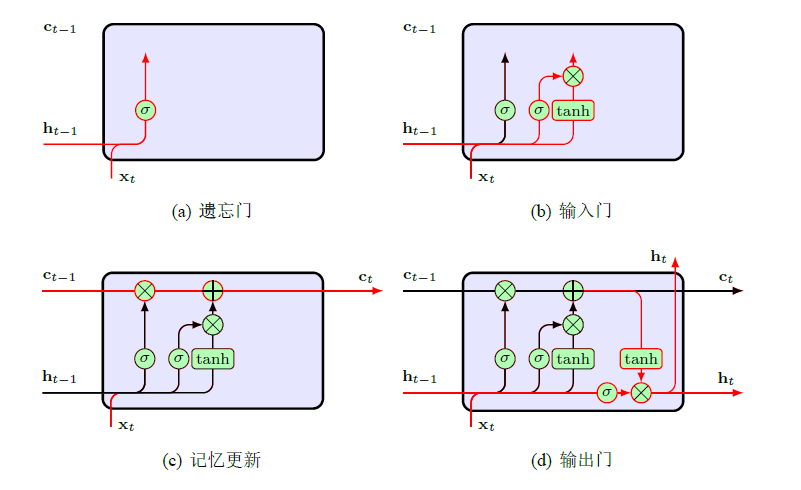
\includegraphics[width=0.9\textwidth]{LSTM.png}
\caption{LSTM 中的门控结构}
\end{figure}
LSTM结构的三部分:
\paragraph{遗忘} 通过遗忘门实现.
$f_t=\sigma (W_f h_{t-1, x_t}+b_f)$$ W_f $权值, $b_f$偏置, 该公式是对$[h_{t−1}, x_t]$ 进行变换, 并得到一个实数向量$f_t$. $f_t$ 的每一维都可以被理解为一个“门”, 它决定可以有多少信息被留下(或遗忘). 

\paragraph{记忆更新}
门控参数$\mathbf{i}_t$
\begin{align*}
    \mathbf{i}_t=\sigma(W[h_t-1, x_t])+b_i \\
    \hat{c}=Than(W_c[h_{t-1}, x_t]+b_i])
    \end{align*}

当前需记忆信息, 记为$\mathbf{i} \cdot \hat{c}_t$

\paragraph{输出}
\begin{align*}
\mathbf{o}_t  & =\sigma(W_o[h_{t-1, x_t]+b_o}) \\
\mathbf{h}_t & ={o}_t \cdot Than(c_t)
\end{align*}
 

\paragraph{循环神经网络和递归神经网络}

循环神经网络(Recurrent NN)是在时间维度上的展开, 代表信息在时间维度从前往后的的传递和积累, 可以类比markov, 后面的信息的概率建立在前面信息的基础上, 在神经网络结构上表现为后面的神经网络的隐藏层的输入是前面的神经网络的隐藏层的输出;有环结构.

递归神经网络(Recursive NN)是空间维度的展开, 是一个树结构, 无环结构.
用循环神经网络(Recurrent NN)来建模的话就是假设句子后面的词的信息和前面的词有关, 而用递归神经网络(Recursive NN)来建模的话, 就是假设句子是一个树状结构, 如由几个部分(主语, 谓语, 宾语)组成.

\subsubsection{LSTM实现}
使用周杰伦歌词, 训练模型并根据前缀“油画”创作⻓度为50个字符的⼀段歌词. 每过40个迭代周期便根据当前训练的模型创作⼀段歌词. 
\begin{figure}[!ht]
    \center
    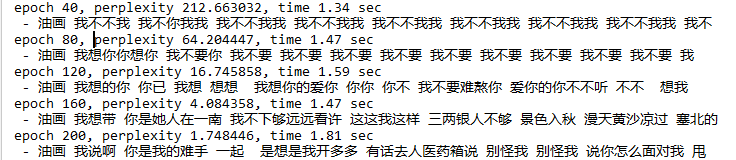
\includegraphics[width=0.8\textwidth]{lyrics.png}
    \end{figure} 
\subsubsection{GRU}
Gated Recurrent Unit (GRU) 门循环单元
\textbf{GRU 中的门控结构}

\begin{figure}[!htb]
\centering
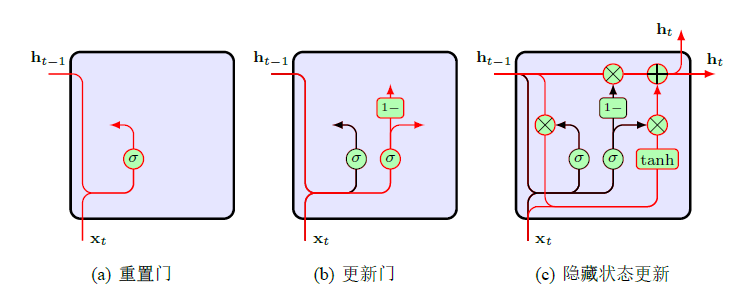
\includegraphics[width=0.9\textwidth]{GRU.png}
\caption{GRU中的门控结构}
\end{figure}

GRU对LSTM进行了简化, 把循环单元状态$h_t$和记忆$c_t$合并为状态$h_t$, 
LSTM传递的两部分信息状态信息$h_{t−1}$和记忆信息$c_{t−1}$. 
GRU有两个门, 
\begin{itemize}
    \item 重置门$r_t$:用来控制前一时刻隐藏状态的记忆程度.
    \item 更新门$u_t$:更新记忆, 使用一个门同时完成遗忘和记忆两种操作, 
\end{itemize}

GRU计算流程:

step1: 更新门$r_t$和重置门$u_t$计算
\begin{align*}
\mathbf{r}_t  & =\sigma(W_r[h_{t-1, x_t]}) \\
\mathbf{u}_t &  =\sigma(W_u[h_{t-1, x_t]})
\end{align*} 

step2: 更新当前隐藏状态 
$$\hat{h}_t=Than(W_h[r_t \cdot h_{t-1}, X_t])$$

step3: 计算更新后的隐藏状态(更新记忆)
$$h_t=(1-u_t) \cdot h_{t-1} + u_t\cdot \hat{h}_t$$

\subsubsection{改进}
\paragraph{双向模型}

\begin{figure}[htp]
    \centering
    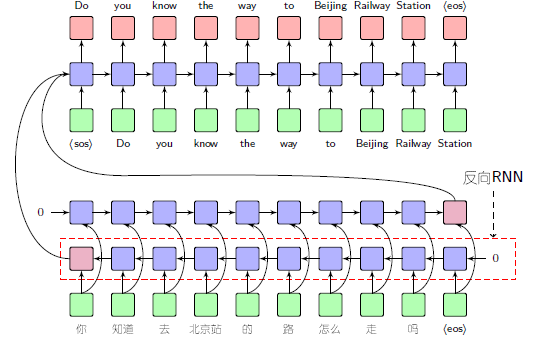
\includegraphics[width=0.9\textwidth]{dual_direction_ML.png}
    \caption{基于双向循环神经网络的机器翻译模型结构}
    \end{figure}
自左向右的模型只考虑了左侧的上下文, 因此可以用自右向左的模型对右侧上下文建模, 最终将两个模型融合同时送给编码端

\begin{figure}[htp]
    \centering
    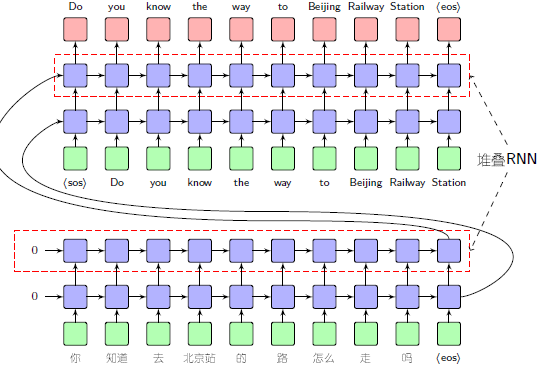
\includegraphics[width=0.9\textwidth]{multiNet_NML.png}
    \caption{基于双层循环神经网络的机器翻译模型结构}
    \end{figure}
 堆叠更多层的网络, 可以提升模型的表示能力
 
\subsection{Attention}

简单的编码器-解码器的问题:
将源语言句子编码为一个实数向量虽然很有效, 但是有明显问题
\begin{itemize}
    \item 
    整个句子编码到一个向量里可能会有信息丢失
    \item 
    缺少源语单词与目标语单词之间的对应. 某种意义上讲, 一个目标语单词的生成无法区分不同源语单词的贡献
\end{itemize}
翻译是具有很强的局部性的, 有些词之间会有更紧密的关系
源语词和目标语词的对应并不是均匀的, 甚至非常稀疏, 比如, 一些短语的生成仅依赖于源文中的少数词, 这些关系可以在表示模型中考虑
\textbf{关注的"局部性"在图像处理、语音识别等领域也有广泛讨论}
\begin{figure}[htp]
    \centering
    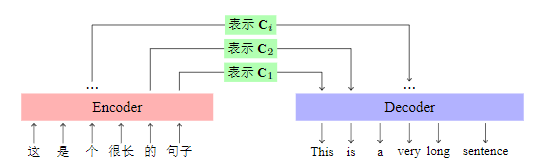
\includegraphics[width=0.9\textwidth]{attention1.png}
    \caption{使用注意力机制的翻译模型}
    \end{figure}
    \paragraph{上下文向量}
可以将注意力机制看做是一种对接收到的信息的加权处理, 上下文向量$\mathbf{C}_j$被定义为对不同时间步编码器输出的状态序列$\{ \mathbf{h}_1,  \mathbf{h}_2, ..., \mathbf{h}_m \}$进行加权求和, 如下:
    \begin{eqnarray}
    \mathbf{C}_j=\sum_{i} \alpha_{i, j} \mathbf{h}_i
    \end{eqnarray}
其中, $\alpha_{i, j}$是{\small\sffamily\bfseries{注意力权重}}\index{注意力权重}(Attention Weight)\index{Attention Weight}, 它表示目标语第$j$个位置与源语第$i$个位置之间的相关性大小. 

\begin{figure}[htp]
    \centering
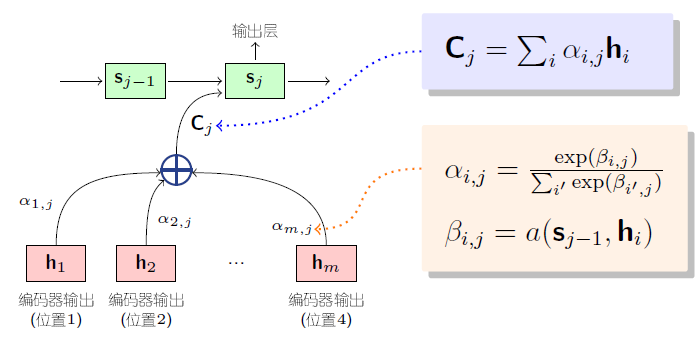
\includegraphics[width=0.9\textwidth]{context_vector_cacl.png}
    \caption{上下文向量计算过程实例}
    \end{figure}

\subsection{Transformer}
使用循环神经网络对源语、目标语建模进行信息提取效果很好, 但是当序列过长时, 词汇之间信息传递距离过长, 导致模型的信息提取能力变差. 
\begin{figure}[htp]
    \centering
    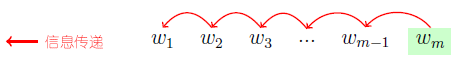
\includegraphics[width=0.9\textwidth]{self-attention1.png}
    \caption{循环神经网络中单词之间的依赖关系}
    \end{figure}
 能否将不同位置之间的词汇间信息传递的距离拉近为1? 
 \begin{figure}[htp]
    \centering
    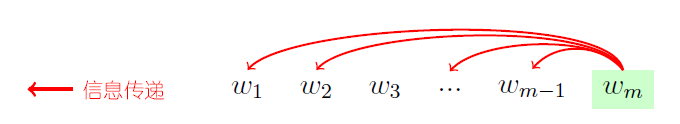
\includegraphics[width=0.9\textwidth]{self_attention2.png}
    \caption{自注意力机制中单词之间的依赖关系}
    \end{figure}


\textbf{自注意力机制(Self-Attention)}可以很好的解决长距离依赖问题, 增强信息抽取能力, 在长距离语言建模任务取得了很好的效果
 自注意力机制则是将源语言每个位置的表示$h_i$看做query, 同时将所有位置的表示看做key和value
 Transformer是Google在2017年提出的一个新型网络结构, 完全基于注意力机制, 取得了很好成绩!通过自注意机制能够直接获取全局信息, 不像RNN需要逐步进行信息提取, 也不像CNN只能获取局部信息, 可以并行化操作, 提高训练效率, Transformer不仅仅被用于神经机器翻译任务, 还广泛用于其他NLP任务、甚至图像处理任务. 
 %----------------------------------------------
\begin{figure}[ht]
    \centering
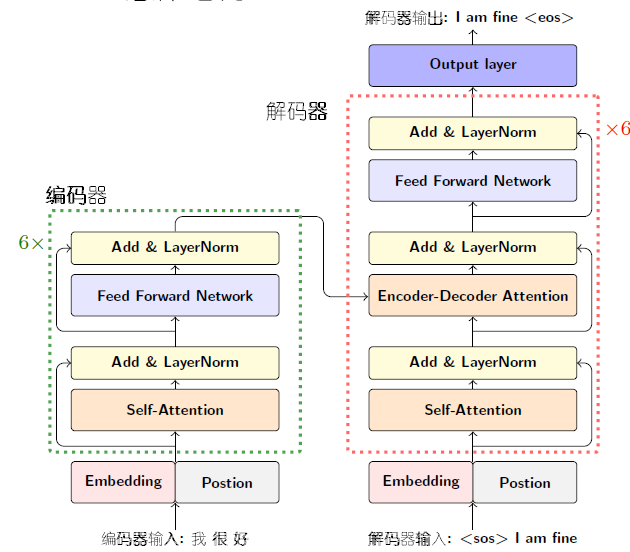
\includegraphics[width=0.9\textwidth]{Transformer1.png}
    \caption{Transformer结构}
    \label{Transformer}
    \end{figure}
    \parinterval 图\ref{Transformer} 展示了经典的Transformer结构. 解码器由若干层组成(绿色虚线框就代表一层). 每一层(layer)的输入都是一个向量序列, 输出是同样大小的向量序列, 而Transformer层的作用是对输入进行进一步的抽象, 得到新的表示结果. 不过这里的层并不是指单一的神经网络结构, 它里面由若干不同的模块组成, 包括:
    \begin{itemize}
        \vspace{0.5em}
        \item {\small\sffamily\bfseries{自注意力子层}}\index{自注意力子层}(Self-attention Sub-layer)\index{Self-attention Sub-layer}:使用自注意力机制对输入的序列进行新的表示;
        \vspace{0.5em}
        \item {\small\sffamily\bfseries{前馈神经网络子层}}\index{前馈神经网络子层}(Feed-forward Sub-layer)\index{Feed-forward Sub-layer}:使用全连接的前馈神经网络对输入向量序列进行进一步变换;
        \vspace{0.5em}
        \item {\small\sffamily\bfseries{残差连接}}\index{残差连接}(Residual Connection, 标记为``Add'')\index{Residual Connection}:对于自注意力子层和前馈神经网络子层, 都有一个从输入直接到输出的额外连接, 也就是一个跨子层的直连. 残差连接可以使深层网络的信息传递更为有效;
        \vspace{0.5em}
        \item {\small\sffamily\bfseries{层正则化}}\index{层正则化}(Layer Normalization)\index{Layer Normalization}:自注意力子层和前馈神经网络子层进行最终输出之前, 会对输出的向量进行层正则化, 规范结果向量取值范围, 这样易于后面进一步的处理. 
        \vspace{0.5em}
        \end{itemize}

\subsubsection{残差连接}
在Transformer中, 编码器、解码器分别由6层网络组成, 每层网络又包含多个子层(自注意力网络、前馈神经网络). Transformer实际上是一个很深的网络结构, 在训练过程中容易出现梯度消失的情况在这里引入了在图像领域用来训练深层网络的技术, 残差网络来避免上述问题.
\begin{eqnarray}
    x_{l+1} = x_l + \mathcal{F} (x_l)
    \end{eqnarray}

    在Transformer的训练过程中, 由于引入了残差操作, 将前面所有层的输出加到一起. 这样会导致高层的参数分布不断变大, 造成训练过程不稳定、训练时间较长. 为了避免这种情况, 在每层中加入了层正则化操作I 使用均值和方差对样本进行平移缩放, 将数据规范化为均值为0, 方差为1的标准分布
    \begin{eqnarray}
        \textrm{LN}(x) = g \cdot \frac{x- \mu} {\sigma} + b
        \end{eqnarray}  


\subsubsection{机器翻译系统简介}


基于规则、基于统计、基于实例、神经网络方法
不同机器翻译方法有不同的特点.  
\begin{enumerate}
    \item 规则系统需要人工书写规则并维护, 人工代价较高. 统计和神经网络方法仅需要设计特征或者神经网络结构, 对人工依赖较少(语言相关的). 
    \item 基于实例、统计和神经网络的方法都需要依赖语料库(数据), 其中统计和神经网络方法具有一定的抗噪能力, 因此也更适合大规模数据情况下的机器翻译系统研发. 
    \item  基于规则和基于实例的方法在受限场景下有较好的精度, 但是在开放领域的翻译上统计和神经网络方法更具优势. 
\end{enumerate}

\begin{table}  [!htb]
    \Large  
    \caption{不同机器翻译方法的对比}  
    \begin{center}  
    \begin{tabular}{l|lll l}  
    \hline  
    &规则&实例&统计&神经 \\ \hline
    人工写规则&是&否&否&否\\ 
    人工代价&高&一般&几乎没有&几乎没有\\ 
    数据驱动&否&是&是&是\\ 
    依赖数据质量&N/A&高&低&较低\\ 
    抗噪声能力&低&低&高&较高\\ 
    使用范围&受限领域&受限领域&通用领域&通用领域\\ 
    翻译精度&高&较高&不确定&不确定\\  
    \hline  
    \end{tabular}  
    \end{center}  
    \end{table}

\subsection{基于梯度的方法的改进}
 \subsubsection{动量法Momentum}
 对于普通的梯度下降法 $\theta \leftarrow \theta - \eta \nabla f(x)$,  当接近最优值时梯度会比较小, 由于学习率固定, 普通的梯度下降法的收敛速度会变慢, 有时甚至陷入局部最优.   
设时间步$t$的自变量为${x}_t$, 学习率为$\eta_t$. 
在时间步$0$, 动量法创建速度变量$\mathbf{v}_0$, 并将其元素初始化成0. 在时间步$t>0$, 动量法对每次迭代的步骤做如下修改:
 $$
 \begin{aligned}
 \mathbf{v}_t &\leftarrow \gamma \mathbf{v}_{t-1} + \eta_t \mathbf{g}_t,  \\
 \mathbf{x}_t &\leftarrow \mathbf{x}_{t-1} - \mathbf{v}_t, 
 \end{aligned}
 $$
 其中$\mathbf{g}_t$同小批量随机梯度中的定义.

 \paragraph{指数加权移动平均exponentially weighted moving average}
 给定超参数$0 \leq \gamma < 1$, 当前时间步$t$的变量$y_t$是上一时间步$t-1$的变量$y_{t-1}$和当前时间步另一变量$x_t$的线性组合:
 $$y_t = \gamma y_{t-1} + (1-\gamma) x_t.$$

对$y_t$展开:

 $$
 \begin{aligned}
 y_t  &= (1-\gamma) x_t + \gamma y_{t-1}\\
          &= (1-\gamma)x_t + (1-\gamma) \cdot \gamma x_{t-1} + \gamma^2y_{t-2}\\
          &= (1-\gamma)x_t + (1-\gamma) \cdot \gamma x_{t-1} + (1-\gamma) \cdot \gamma^2x_{t-2} + \gamma^3y_{t-3}\\
          &\ldots
 \end{aligned}
 $$
 
 令$n = 1/(1-\gamma)$, 那么 $\left(1-1/n\right)^n = \gamma^{1/(1-\gamma)}$. 
 
 $$ \lim_{n \rightarrow \infty}  \left(1-\frac{1}{n}\right)^n = \exp(-1) \approx 0.3679, $$
 当$\gamma \rightarrow 1$时, $\gamma^{1/(1-\gamma)}=\exp(-1)$, 如$0.95^{20} \approx \exp(-1)$. 如果把$\exp(-1)$当作一个比较小的数, 我们可以在近似中忽略所有含$\gamma^{1/(1-\gamma)}$以及更高阶的系数的项.  
 $y_t$可看作是对最近$1/(1-\gamma)$个时间步的$x_t$值的加权平均. 


对动量法的速度变量做变形:

 $$\mathbf{v}_t \leftarrow \gamma \mathbf{v}_{t-1} + (1 - \gamma) \left(\frac{\eta_t}{1 - \gamma} \mathbf{g}_t\right). $$
$\mathbf{v}_t$实际上对序列$\{\eta_{t-i}\mathbf{g}_{t-i} /(1-\gamma):i=0, \ldots, 1/(1-\gamma)-1\}$做了指数加权移动平均. 在动量法中, 自变量在各个方向上的移动幅度同时取决于当前梯度和过去的各个梯度在各个方向上是否一致. 

若用 $G_t$表示第t轮迭代的动量,  $g_t$表示第t轮迭代的更新量, 当 $t \to \infty $,  $G_t= \frac{g_0}{1-\gamma} $, 如果梯度保持不变, 最终的更新速度会是梯度项乘以学习率的 $\frac{1}{1-r}$ 倍. 

\subsubsection{AdaGrad}
\paragraph{问题} 假设目标函数为$f$, 自变量为一个二维向量$[x_1,  x_2]^\top$, $x_1, x_2$在迭代时都使用相同的学习率. 若两者梯度值差别较大, 选择一个小学习率会使在梯度值较小的维度迭代过慢. 
\paragraph{解决方法}: 不同维度设置不同学习率. 

AdaGrad算法使用一个小批量随机梯度$\mathbf{g}_t$按元素平方的累加变量$\mathbf{s}_t$.  $\mathbf{s}_0$中每个元素初始化为0. 在$t$时刻, 累积平方梯度:
$$\mathbf{s}_t \leftarrow \mathbf{s}_{t-1} + \mathbf{g}_t \odot \mathbf{g}_t, $$
其中$\odot$是按元素相乘. 
之后, 将自变量中每个元素的学习率通过按元素运算重新调整:
$$\mathbf{x}_t \leftarrow \mathbf{x}_{t-1} - \frac{\eta}{\sqrt{\mathbf{s}_t + \epsilon}} \odot \mathbf{g}_t, $$
其中$\epsilon$是为了维持数值稳定性而添加的常数.  

\subsubsection{RMSProp}
\textbf{问题}: 因为调整学习率时分⺟上的变量$s_t$⼀直在累加按元素平方的小批量随机梯度, 所以⽬标函数⾃变量每个元素的学习率在迭代过程中⼀直在降低(或不变). 因此, 当学习率在迭代早期降得较快且当前解依然不佳时, AdaGrad算法在迭代后期由于学习率过小, 可能较难找到一个有用的解. 

 \textbf{解决方法:} 改变Adagrad梯度积累为指数加权的移动平均. 
 
给定超参数$0 \leq \gamma < 1$, RMSProp算法在时间步$t>0$计算

$$\mathbf{s}_t \leftarrow \gamma \mathbf{s}_{t-1} + (1 - \gamma) \mathbf{g}_t \odot \mathbf{g}_t. $$

将目标函数自变量中每个元素的学习率通过按元素运算重新调整, 然后更新自变量

$$\mathbf{x}_t \leftarrow \mathbf{x}_{t-1} - \frac{\eta}{\sqrt{\mathbf{s}_t + \epsilon}} \odot \mathbf{g}_t,  $$

其中$\epsilon$是为了维持数值稳定性而添加的常数. 自变量每个元素的学习率在迭代过程中就不再一直降低(或不变). 
\subsubsection{AdaDelta}
\paragraph{问题:}同RMSProp待解决问题相同 \\
\textbf{解决方法:}不设置学习率, 用一阶的方法, 近似模拟二阶牛顿法. 使用了小批量随机梯度$\mathbf{g}_t$按元素平方的指数加权移动平均变量$\mathbf{s}_t$. 

在时间步0, 它的所有元素被初始化为0. 给定超参数$0 \leq \rho < 1$], 

在时间步$t>0$
$$\mathbf{s}_t \leftarrow \rho \mathbf{s}_{t-1} + (1 - \rho) \mathbf{g}_t \odot \mathbf{g}_t. $$

状态变量$\Delta\mathbf{x}_t$, 在时间步0时被初始化为0. $\Delta\mathbf{x}_{t-1}$是来计算自变量的变化量:

$$ \mathbf{g}_t' \leftarrow \sqrt{\frac{\Delta\mathbf{x}_{t-1} + \epsilon}{\mathbf{s}_t + \epsilon}}   \odot \mathbf{g}_t,  $$

其中$\epsilon$是为了维持数值稳定性而添加的常数, 如$10^{-5}$. 

更新自变量:
$$\mathbf{x}_t \leftarrow \mathbf{x}_{t-1} - \mathbf{g}'_t. $$

最后, $\mathbf{g}'_t$按元素平方的指数加权移动平均:
$$\Delta\mathbf{x}_t \leftarrow \rho \Delta\mathbf{x}_{t-1} + (1 - \rho) \mathbf{g}'_t \odot \mathbf{g}'_t. $$

可以看到, 如不考虑$\epsilon$的影响, AdaDelta算法与RMSProp算法的不同之处在于使用$\sqrt{\Delta\mathbf{x}_{t-1}}$来替代超参数$\eta$. 

\subsubsection{Adam} \citep{Kingma2014Adam}
Adam可以理解为加了Momentum 的 RMSprop, 然后修正偏差.
\begin{figure}[htp]
    \centering
     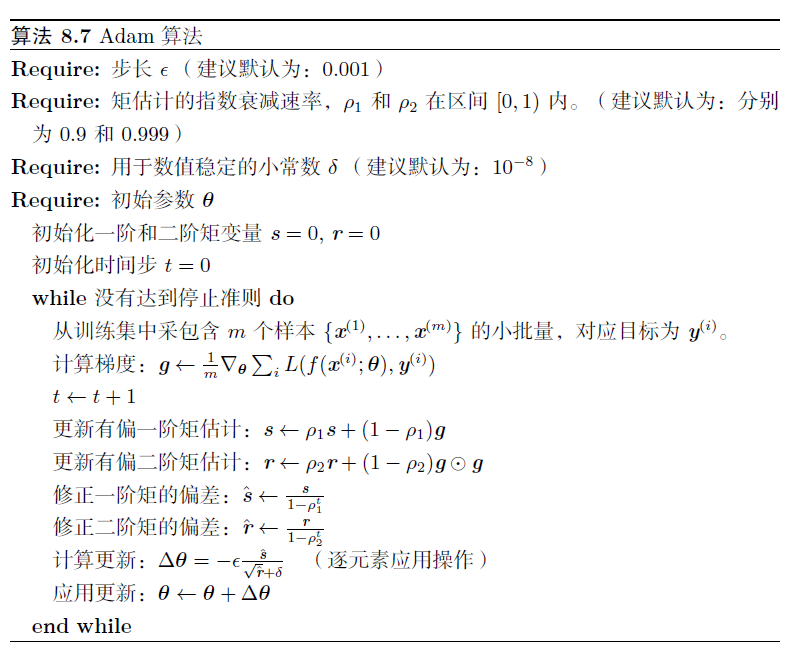
\includegraphics[width=0.8\textwidth]{adam.png}
 
    \label{fig:adm}
    \end{figure}

\subsection{建模}

\parinterval 在给定源语言句子$\mathbf{x}$的情况下, 找出翻译概率最大的目标语译文$\hat{\mathbf{y}}$:
\begin{eqnarray}
\hat{\mathbf{y}} = \argmax_{\mathbf{y}} \textrm{P} (\mathbf{y} | \mathbf{x})
\end{eqnarray}

\noindent 这里, 用$\mathbf{x}=\{ x_1, x_2, ...,  x_m \}$表示输入的源语言单词序列, $\mathbf{y}=\{ y_1, y_2, ...,  y_n \}$ 表示生成的目标语单词序列. 由于神经机器自左向右逐词翻译, 并且考虑之前的结果, 因此对$\textrm{P} (\mathbf{y} | \mathbf{x})$的求解可以转换为:
\begin{eqnarray}
\textrm{P} (\mathbf{y} | \mathbf{x}) = \prod_{j=1}^{n} \textrm{P} ( y_j | \mathbf{y}_{<j },  \mathbf{x}  )
\end{eqnarray}
$ \mathbf{y}_{<j }$表示目标语第$j$个位置之前已经生成的译文单词序列. 

\parinterval 求解$\textrm{P}(y_j | \mathbf{y}_{<j}, \mathbf{x})$有三个关键问题(图\ref{fig:probquestion}):

\begin{itemize}
\item	{\small\sffamily\bfseries{词嵌入}}(Word Embedding):$\mathbf{x}$和$\mathbf{y}_{<j }$的分布式表示. 将源语言单词转化为实数向量. 可以把这个过程记为$\textrm{e}_x (\cdot)$. 类似的, $\mathbf{y}_{<j }$记为$\textrm{e}_y (\cdot)$. 
\item	在词嵌入的基础上获取整个序列的表示, 即句子的{\small\sffamily\bfseries{表示学习}}(Representation Learning). 如图\ref{fig:probquestion}中, 编码器最后一个循环单元的输出$\mathbf{h}_m$被看作是一种包含了源语句子信息的表示结果, 记为$\mathbf{C}$. 
\item	得到每个目标语单词的概率, 即译文单词的{\small\sffamily\bfseries{生成}}Generation). 可以用一个Softmax输出层来获取当前时刻所有单词的分布.令目标语序列$j$时刻的循环神经网络的输出向量(或状态)为$\mathbf{s}_j$. $ y_j$的生成只依赖前一个状态$\mathbf{s}_{j-1}$和当前时刻的输入. 同时考虑源语言信息$\mathbf{C}$, $\textrm{P}(y_j  | \mathbf{y}_{<j}, \mathbf{x})$可以被重新定义为:
\begin{eqnarray}
\textrm{P} (y_j | \mathbf{y}_{<j}, \mathbf{x}) \equiv \textrm{P} ( {y_j | \mathbf{s}_{j-1} , y_{j-1}, \mathbf{C}} )
\end{eqnarray}
可以进一步简化为, 
\begin{eqnarray}
\textrm{P} (y_j | \mathbf{y}_{<j}, \mathbf{x}) \equiv
 \left \{ \begin{array}{ll}
\textrm{P} (y_j |\mathbf{C} , y_{j-1}) &j=1 \\
\textrm{P} (y_j|\mathbf{s}_{j-1}, y_{j-1})  \quad &j>1
\end{array} \right . 
\end{eqnarray}
\end{itemize}

\begin{figure}[htp]
    \centering
     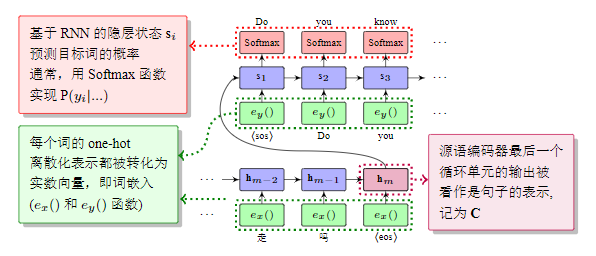
\includegraphics[width=0.8\textwidth]{RNNprobquestion.png}
    \caption{求解$\textrm{P} (y_j | \mathbf{y}_{<j}, \mathbf{x})$的三个基本问题}
    \label{fig:probquestion}
    \end{figure}

\begin{figure}[htp]
\centering
    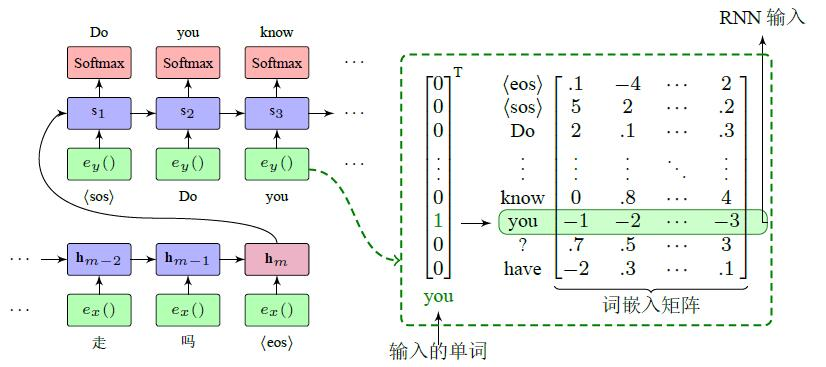
\includegraphics[width=0.8\textwidth]{figures/MachineTranslation/fig6-12.jpg}
\caption{词嵌入的生成过程}
\label{fig:genWordEmbedded}
\end{figure}

    \parinterval 如何在神经机器翻译系统中获得单词的词嵌入表示?这里引入一个词嵌入层对输入的单词进行词嵌入表示, 即图\ref{fig:genWordEmbedded}中的绿色方框部分. 假设输入的单词$y_j$已经被表示为One-hot形式(行向量). 词嵌入层的工作就是把One-hot向量右乘一个实数矩阵$\mathbf{E}$, 得到的结果(行向量)就是这个单词所对应的词嵌入结果. 
    \begin{eqnarray}
    \textrm{e}_y (y_j) = y_j \mathbf{E} 
    \end{eqnarray} 

    \noindent 这里, $\mathbf{E}$也被称作词嵌入矩阵, 它可以作为模型的一部分参数共同参与机器翻译系统的训练, 也可以由外部其他模块训练得到(如预训练模型). $\mathbf{E}$的大小为$|V| \times d$, 这里$|V|$表示词表$V$的大小, $d$表示循环神经网络输入和输出向量的维度. 
    

    词嵌入的作用是把离散化的单词表示转换为连续空间上的分布式表示
    \begin{enumerate}
        \item   把输入的词转换成唯一对应的词表大小的0-1向量
        \item 根据0-1向量, 从词嵌入矩阵中取出对应的词嵌入$e(\cdot)$
        \item 取出的词嵌入$e(\cdot)$作为循环神经网络的输入
    \end{enumerate} 
  
    
    
\begin{figure}[htp]
    \centering
    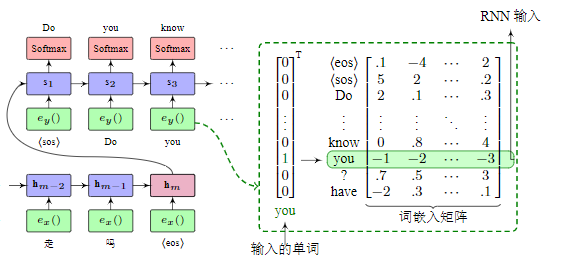
\includegraphics[width=0.8\textwidth]{NMLEmbed.png}
    \caption{词嵌入的生成过程}
 
    \end{figure}

输出层需要得到每个目标语单词的生成概率, 进而选取概率最高的词作为输出. 但RNN中的隐藏层并不会输出单词概率, 而是输出s, 其每一行对应一个单词表示.
s经过权重矩阵W变成$\hat{s}$, 其隐藏层维度变换成词表的大小
$\hat{s}$经过Softmax变换得到不同词作为输出的概率, 即单词i的概率
$$p_i= Softmax(i) = \frac{{e^{\hat{s}_i}}}{{\sum_j e^{\hat{s}_j}}}$$
 


    \begin{figure}[htp]
        \centering
        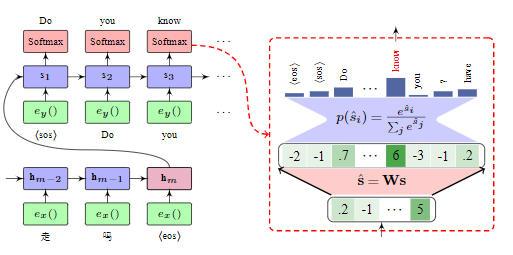
\includegraphics[width=0.8\textwidth]{outputpredict.png}
        \caption{输出层的预测过程} 
        \end{figure}

\subsubsection{RNN训练}
训练RNN我们通常会使用Adam或者SGD两种优化器, 它们各有优劣. Adam 通用, 性能不是最好, SGD  一个任务一个配置, 效果更好. 
因此需要快速得到模型看一下初步效果, 选择Adam. 
若是需要在一个任务上得到最优的结果, 选择SGD. 
需要注意的是, 训练RNN的时候, 我们通常会遇到梯度爆炸的问题, 也就是梯度突然变得很大, 这种情况下需要使用梯度裁剪来防止梯度超过阈值. 